\documentclass{article}
\usepackage[utf8]{inputenc}
\usepackage[page]{appendix}
\usepackage{graphicx}
\usepackage{booktabs}
\usepackage{lscape}
\usepackage{biblatex}
\usepackage{longtable}
\usepackage{geometry}
\usepackage{mathtools,amsmath,amsfonts}
\usepackage{subcaption}
\usepackage{wrapfig}

\addbibresource{refs.bib}
\graphicspath{ {plots/} }


\begin{document}	

\begin{center}
\rule{\textwidth}{.4pt}
\Large{SAT solutions for 3D Sudokus\\\vspace{.2cm}}
\rule{\textwidth}{.8pt}

\small{Freek Boutkan 10004616\\Jochem Barelds 5795567}
\end{center}

\begin{abstract}
3D sudokus are a generalization of the classic 2D sudoku to three dimensions. We examine the relation between the relative number of prefilled cells needed to solve a 3D sudoku. The hypothesis is "as the size of a 3D sudoku grows, the relative number of givens needed to find a solution also increases". 3D sudoku's of diffent sizes and with varying degrees of prefilled cells were generated and encoded in CNF. Minisat was used to solve the puzzle. Conflict and decision statistics were used to determine if the puzzle could be solved solely by logical inferences. The hypothesis is accepted although future work could provide more insight in the exact number of givens needed.
\end{abstract}

\documentclass[11pt]{article}
%Gummi|065|=)
\usepackage{mathtools,amsmath,amsfonts}
\begin{document}

\section{Definitions}

A 3D Sudoku is a Sudoku of size $N \times N \times N$. It consists of rows, columns, and layers, which are sequences of cells spanning across a single dimension. Similar to the 2D Sudoku, each row, column, and layer must contain every number $d \in \{1, \hdots, N\}$ exactly once. In contrast to 2D Sudokus, the constraint that every number must also appear exactly once in each block is dropped for the 3D Sudoku. 

\end{document}


% rules
% why interesting
% hypothesis
% maybe add image of 3D sudoku

\section{Encoding}
Since symbols in propositional logic can only be true or false it is not possible to encode the number of a cell with a single symbol. For a $N$ sized sudoku there are $N$ different posible digits for each cell. Thus for a single cell $N$ different symbols are needed. In this paper the sentence 'Position $x$, $y$, $z$ contains a $d$' is encoded as follows:
\begin{align}
  p_{xyz}^d &= 1
\end{align}
We have adopted Webers \cite{weber2005sat} encoding for this experiment. Webers encoding consists of the following elements
\begin{enumerate}
  \item At least one of $N$ digits in a cell. This can be encoded as a single clause of length $N$
    \begin{align}
      \bigvee_{d=1}^N p_{xyz}^d
    \end{align}
  \item At most one of $N$ digits in a cell. This can be encoded as $\sum_{n=1}^{N-1}n$ binary clauses:
    \begin{align}
      \bigwedge_{1 \leq d < d' \leq N}^N \neg p_{xyz}^d \vee \neg p_{xyz}^{d'}
    \end{align}
  \item Validity of $N$ positions. Weber defines a row (or column or region) of $N$ cells as valid if all the cells contain distinct values. This is true because there are just as many digits as cells. This can be encoded using $N \cdot \sum_{n=1}^{N-1}n$ binary clauses:
    \begin{align}
      \text{Valid}(p_1,\dots,p_N) \implies \bigwedge_{1 \leq i < i' \leq N}\bigwedge_{d=1}^N \neg p_{i}^d \vee \neg p_{i'}^{d}
    \end{align}
\end{enumerate}

\subsection{Number of clauses and average length}
For each of the $N^3$ cells an 'At least one` and an 'At most one` clause is needed. Also for each dimension (row/column/layer) $N^2$ valid clauses are needed. Given an empty 3D sudoku of size $N$ the number of clauses $c$ needed to represent the puzzle is given by equation \ref{eq_clauses} and the average length of the clauses by equation \ref{eq_clauses_avg_length}. Since most of clauses are of length two the average length of the clause decreases as N grows, as can be seen in figure \ref{fig_dimecs_props}. As N increases the number of binary clauses becomes bigger. For a large $N$ the average length approximates 2, but the distribution of the clause lenghts is very uneven. The length of the clauses can be relevant for SAT solvers since 2-SAT problems can be solved in polynomial time and this is also the case for some close to 2-SAT problems.

\subsection{Givens}
All the given (prefilled) cells can simply be added to the list of clauses. For those cells 'at least one` and 'at most one` clauses are not necessary as long as the negation for all the other number in the same cell are also added. This reduces the number of clauses needed to describe the puzzle drastically, especially for bigger puzzles with a high number of givens. For this paper both encodings are implemented and tested. The more sophisticated encoding method is referred to as smart and the more naive encoding is referred to as not smart.
\begin{align}
  \label{eq_clauses}
  c(N) = N^3 + N^3 \sum_{n=1}^{N-1}n + 3N^3\sum_{n=1}^{N-1}n = N^3(1 + 4\sum_{n=1}^{N-1}n)
\end{align}
\begin{align}
  \label{eq_clauses_avg_length}
  l(N) = \frac{N\cdot N^3 + 2\cdot4 N^3 \sum_{n=1}^{N-1}}{N^3(1 + 4\sum_{n=1}^{N-1})} = \frac{8N\sum_{n=1}^{N-1}}{4\sum_{n=1}^{N-1}+1}
\end{align}

\begin{figure}
  \centering
  \label{fig_dimecs_props}
  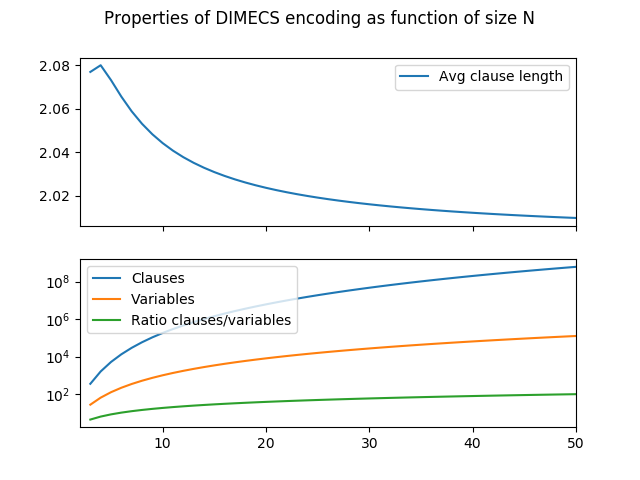
\includegraphics[width=.6\textwidth]{dimecs_props}
  
  \caption{Properties of DIMECS encoding}
\end{figure}


\section{Experimental Setup}
% how do we measure complexity
% what software do we use, completely describe all the tools and procedures
% maybe insert figure from Finns paper

\subsection{Dataset}
% exlain we needed to write our own algorithm to generate 3d sudoku's of different sizes


% tabel with all avg/stddev 
% heatmap
% some plots


\section{Results and Analysis}
% differenses Smart vs NotSmorrt
% explain how low/hight M/N influences complexity
% how do the results accept/reject our hypotheses

\section{Conclusion and Future Work}
% Now tthat the experiment is done: did the hpyotheses make any sense, is it meaning full
% possible future work: investige exact M/N ratio for different size, can this research be generalized to n-Dimensional sudoku;s


\begin{appendices}
\newgeometry{margin=.75cm}
\section{Full results}
\begin{landscape}
\begin{small}
\begin{longtable}[c]{@{}lll|ll|ll|ll|ll|lll@{}}
\toprule
N  & M  & Smart & \multicolumn{2}{c}{propagations} & \multicolumn{2}{c}{decisions} & \multicolumn{2}{c}{cpu\_time} & \multicolumn{2}{c}{conflicts} & \multicolumn{2}{c}{clauses} &  \\* 
   &    &       & mean            & std            & mean          & std           & mean          & std           & mean          & std           & mean          & std         &  \\
  \midrule
\endfirsthead
%
\endhead
%
\bottomrule
\endfoot
%
\endlastfoot
%
3  & 10 & True  & 106.2           & 56.35          & 3.2           & 1.3           & 0.0           & 0.0           & 0.6           & 1.34          & 272.4         & 12.93       &  \\
   &    & False & 106.2           & 56.35          & 3.2           & 1.3           & 0.0           & 0.0           & 0.6           & 1.34          & 449.4         & 92.22       &  \\
   & 20 & True  & 81.0            & 0.0            & 1.0           & 0.0           & 0.0           & 0.0           & 0.0           & 0.0           & 178.4         & 7.06        &  \\
   &    & False & 81.0            & 0.0            & 1.0           & 0.0           & 0.0           & 0.0           & 0.0           & 0.0           & 178.4         & 7.06        &  \\
   & 30 & True  & 81.0            & 0.0            & 1.0           & 0.0           & 0.0           & 0.0           & 0.0           & 0.0           & 127.6         & 11.46       &  \\
   &    & False & 81.0            & 0.0            & 1.0           & 0.0           & 0.0           & 0.0           & 0.0           & 0.0           & 127.6         & 11.46       &  \\
   & 40 & True  & 81.0            & 0.0            & 1.0           & 0.0           & 0.0           & 0.0           & 0.0           & 0.0           & 108.4         & 6.43        &  \\
   &    & False & 81.0            & 0.0            & 1.0           & 0.0           & 0.0           & 0.0           & 0.0           & 0.0           & 108.4         & 6.43        &  \\
   & 50 & True  & 81.0            & 0.0            & 1.0           & 0.0           & 0.0           & 0.0           & 0.0           & 0.0           & 81.6          & 6.27        &  \\
   &    & False & 81.0            & 0.0            & 1.0           & 0.0           & 0.0           & 0.0           & 0.0           & 0.0           & 81.6          & 6.27        &  \\
   & 60 & True  & 81.0            & 0.0            & 1.0           & 0.0           & 0.0           & 0.0           & 0.0           & 0.0           & 53.0          & 2.55        &  \\
   &    & False & 81.0            & 0.0            & 1.0           & 0.0           & 0.0           & 0.0           & 0.0           & 0.0           & 53.0          & 2.55        &  \\
   & 70 & True  & 81.0            & 0.0            & 1.0           & 0.0           & 0.0           & 0.0           & 0.0           & 0.0           & 43.2          & 2.59        &  \\
   &    & False & 81.0            & 0.0            & 1.0           & 0.0           & 0.0           & 0.0           & 0.0           & 0.0           & 43.2          & 2.59        &  \\
   & 80 & True  & 81.0            & 0.0            & 1.0           & 0.0           & 0.0           & 0.0           & 0.0           & 0.0           & 26.6          & 0.89        &  \\
   &    & False & 81.0            & 0.0            & 1.0           & 0.0           & 0.0           & 0.0           & 0.0           & 0.0           & 26.6          & 0.89        &  \\
   & 90 & True  & 81.0            & 0.0            & 1.0           & 0.0           & 0.0           & 0.0           & 0.0           & 0.0           & 12.0          & 0.0         &  \\
   &    & False & 81.0            & 0.0            & 1.0           & 0.0           & 0.0           & 0.0           & 0.0           & 0.0           & 12.0          & 0.0         &  \\
  \midrule
4  & 10 & True  & 290.0           & 52.73          & 7.4           & 3.13          & 0.0           & 0.0           & 0.6           & 0.89          & 1157.8        & 45.52       &  \\
   &    & False & 290.0           & 52.73          & 7.4           & 3.13          & 0.0           & 0.0           & 0.6           & 0.89          & 1949.8        & 200.05      &  \\
   & 20 & True  & 256.0           & 0.0            & 2.4           & 1.14          & 0.0           & 0.0           & 0.0           & 0.0           & 845.0         & 16.99       &  \\
   &    & False & 256.0           & 0.0            & 2.4           & 1.14          & 0.0           & 0.0           & 0.0           & 0.0           & 926.8         & 110.87      &  \\
   & 30 & True  & 256.0           & 0.0            & 1.2           & 0.45          & 0.0           & 0.0           & 0.0           & 0.0           & 585.8         & 15.58       &  \\
   &    & False & 256.0           & 0.0            & 1.2           & 0.45          & 0.0           & 0.0           & 0.0           & 0.0           & 593.8         & 30.77       &  \\
   & 40 & True  & 256.0           & 0.0            & 1.0           & 0.0           & 0.0           & 0.0           & 0.0           & 0.0           & 425.6         & 20.34       &  \\
   &    & False & 256.0           & 0.0            & 1.0           & 0.0           & 0.0           & 0.0           & 0.0           & 0.0           & 425.6         & 20.34       &  \\
   & 50 & True  & 256.0           & 0.0            & 1.0           & 0.0           & 0.0           & 0.0           & 0.0           & 0.0           & 324.2         & 14.67       &  \\
   &    & False & 256.0           & 0.0            & 1.0           & 0.0           & 0.0           & 0.0           & 0.0           & 0.0           & 324.2         & 14.67       &  \\
   & 60 & True  & 256.0           & 0.0            & 1.0           & 0.0           & 0.0           & 0.0           & 0.0           & 0.0           & 233.0         & 15.35       &  \\
   &    & False & 256.0           & 0.0            & 1.0           & 0.0           & 0.0           & 0.0           & 0.0           & 0.0           & 233.0         & 15.35       &  \\
   & 70 & True  & 256.0           & 0.0            & 1.0           & 0.0           & 0.0           & 0.0           & 0.0           & 0.0           & 168.4         & 5.68        &  \\
   &    & False & 256.0           & 0.0            & 1.0           & 0.0           & 0.0           & 0.0           & 0.0           & 0.0           & 168.4         & 5.68        &  \\
   & 80 & True  & 256.0           & 0.0            & 1.0           & 0.0           & 0.0           & 0.0           & 0.0           & 0.0           & 100.6         & 5.46        &  \\
   &    & False & 256.0           & 0.0            & 1.0           & 0.0           & 0.0           & 0.0           & 0.0           & 0.0           & 100.6         & 5.46        &  \\
   & 90 & True  & 256.0           & 0.0            & 1.0           & 0.0           & 0.0           & 0.0           & 0.0           & 0.0           & 51.2          & 1.48        &  \\
   &    & False & 256.0           & 0.0            & 1.0           & 0.0           & 0.0           & 0.0           & 0.0           & 0.0           & 51.2          & 1.48        &  \\
  \midrule
5  & 10 & True  & 6101.0          & 7316.34        & 100.2         & 100.42        & 0.0           & 0.0           & 58.8          & 73.64         & 3751.8        & 41.08       &  \\
   &    & False & 6129.8          & 7378.52        & 103.6         & 107.67        & 0.0           & 0.0           & 60.4          & 77.1          & 6539.2        & 191.67      &  \\
   & 20 & True  & 625.0           & 0.0            & 1.0           & 0.0           & 0.0           & 0.0           & 0.0           & 0.0           & 2534.2        & 113.93      &  \\
   &    & False & 625.0           & 0.0            & 1.0           & 0.0           & 0.0           & 0.0           & 0.0           & 0.0           & 2534.2        & 113.93      &  \\
   & 30 & True  & 625.0           & 0.0            & 1.0           & 0.0           & 0.0           & 0.0           & 0.0           & 0.0           & 1818.8        & 72.25       &  \\
   &    & False & 625.0           & 0.0            & 1.0           & 0.0           & 0.0           & 0.0           & 0.0           & 0.0           & 1818.8        & 72.25       &  \\
   & 40 & True  & 625.0           & 0.0            & 1.0           & 0.0           & 0.0           & 0.0           & 0.0           & 0.0           & 1313.4        & 71.02       &  \\
   &    & False & 625.0           & 0.0            & 1.0           & 0.0           & 0.0           & 0.0           & 0.0           & 0.0           & 1313.4        & 71.02       &  \\
   & 50 & True  & 625.0           & 0.0            & 1.0           & 0.0           & 0.0           & 0.0           & 0.0           & 0.0           & 996.4         & 17.84       &  \\
   &    & False & 625.0           & 0.0            & 1.0           & 0.0           & 0.0           & 0.0           & 0.0           & 0.0           & 996.4         & 17.84       &  \\
   & 60 & True  & 625.0           & 0.0            & 1.0           & 0.0           & 0.0           & 0.0           & 0.0           & 0.0           & 729.4         & 20.03       &  \\
   &    & False & 625.0           & 0.0            & 1.0           & 0.0           & 0.0           & 0.0           & 0.0           & 0.0           & 729.4         & 20.03       &  \\
   & 70 & True  & 625.0           & 0.0            & 1.0           & 0.0           & 0.0           & 0.0           & 0.0           & 0.0           & 520.4         & 34.12       &  \\
   &    & False & 625.0           & 0.0            & 1.0           & 0.0           & 0.0           & 0.0           & 0.0           & 0.0           & 520.4         & 34.12       &  \\
   & 80 & True  & 625.0           & 0.0            & 1.0           & 0.0           & 0.0           & 0.0           & 0.0           & 0.0           & 301.8         & 5.76        &  \\
   &    & False & 625.0           & 0.0            & 1.0           & 0.0           & 0.0           & 0.0           & 0.0           & 0.0           & 301.8         & 5.76        &  \\
   & 90 & True  & 625.0           & 0.0            & 1.0           & 0.0           & 0.0           & 0.0           & 0.0           & 0.0           & 150.0         & 3.08        &  \\
   &    & False & 625.0           & 0.0            & 1.0           & 0.0           & 0.0           & 0.0           & 0.0           & 0.0           & 150.0         & 3.08        &  \\
  \midrule
6  & 10 & True  & 525034.0        & 58329.24       & 8156.5        & 306.18        & 0.09          & 0.01          & 4102.5        & 212.84        & 9588.5        & 40.31       &  \\
   &    & False & 1832970.33      & 2265787.61     & 24530.67      & 28361.71      & 0.49          & 0.7           & 13828.67      & 16846.89      & 16893.0       & 192.19      &  \\
   & 20 & True  & 1468.2          & 176.47         & 12.6          & 8.26          & 0.0           & 0.0           & 1.8           & 1.79          & 6750.2        & 124.98      &  \\
   &    & False & 1468.2          & 176.47         & 12.6          & 8.26          & 0.0           & 0.0           & 1.8           & 1.79          & 8737.2        & 1121.59     &  \\
   & 30 & True  & 1296.0          & 0.0            & 1.0           & 0.0           & 0.0           & 0.0           & 0.0           & 0.0           & 4703.6        & 188.09      &  \\
   &    & False & 1296.0          & 0.0            & 1.0           & 0.0           & 0.0           & 0.0           & 0.0           & 0.0           & 4703.6        & 188.09      &  \\
   & 40 & True  & 1296.0          & 0.0            & 1.0           & 0.0           & 0.0           & 0.0           & 0.0           & 0.0           & 3357.0        & 60.66       &  \\
   &    & False & 1296.0          & 0.0            & 1.0           & 0.0           & 0.0           & 0.0           & 0.0           & 0.0           & 3357.0        & 60.66       &  \\
   & 50 & True  & 1296.0          & 0.0            & 1.0           & 0.0           & 0.0           & 0.0           & 0.0           & 0.0           & 2503.6        & 45.34       &  \\
   &    & False & 1296.0          & 0.0            & 1.0           & 0.0           & 0.0           & 0.0           & 0.0           & 0.0           & 2503.6        & 45.34       &  \\
   & 60 & True  & 1296.0          & 0.0            & 1.0           & 0.0           & 0.0           & 0.0           & 0.0           & 0.0           & 1816.6        & 37.77       &  \\
   &    & False & 1296.0          & 0.0            & 1.0           & 0.0           & 0.0           & 0.0           & 0.0           & 0.0           & 1816.6        & 37.77       &  \\
   & 70 & True  & 1296.0          & 0.0            & 1.0           & 0.0           & 0.0           & 0.0           & 0.0           & 0.0           & 1275.6        & 60.58       &  \\
   &    & False & 1296.0          & 0.0            & 1.0           & 0.0           & 0.0           & 0.0           & 0.0           & 0.0           & 1275.6        & 60.58       &  \\
   & 80 & True  & 1296.0          & 0.0            & 1.0           & 0.0           & 0.0           & 0.0           & 0.0           & 0.0           & 800.8         & 13.83       &  \\
   &    & False & 1296.0          & 0.0            & 1.0           & 0.0           & 0.0           & 0.0           & 0.0           & 0.0           & 800.8         & 13.83       &  \\
   & 90 & True  & 1296.0          & 0.0            & 1.0           & 0.0           & 0.0           & 0.0           & 0.0           & 0.0           & 372.6         & 8.11        &  \\
   &    & False & 1296.0          & 0.0            & 1.0           & 0.0           & 0.0           & 0.0           & 0.0           & 0.0           & 372.6         & 8.11        &  \\
  \midrule
7  & 10 & True  & -               & -              & -             & -             & -             & -             & -             & -             & -             & -           &  \\
   &    & False & -               & -              & -             & -             & -             & -             & -             & -             & -             & -           &  \\
   & 20 & True  & 9309.6          & 8541.91        & 111.2         & 111.85        & 0.0           & 0.0           & 49.2          & 58.46         & 15055.2       & 89.97       &  \\
   &    & False & 9309.6          & 8541.91        & 111.2         & 111.85        & 0.0           & 0.0           & 49.2          & 58.46         & 22379.4       & 758.45      &  \\
   & 30 & True  & 2401.0          & 0.0            & 1.0           & 0.0           & 0.0           & 0.0           & 0.0           & 0.0           & 10376.4       & 259.79      &  \\
   &    & False & 2401.0          & 0.0            & 1.0           & 0.0           & 0.0           & 0.0           & 0.0           & 0.0           & 10376.4       & 259.79      &  \\
   & 40 & True  & 2401.0          & 0.0            & 1.0           & 0.0           & 0.0           & 0.0           & 0.0           & 0.0           & 7429.6        & 107.48      &  \\
   &    & False & 2401.0          & 0.0            & 1.0           & 0.0           & 0.0           & 0.0           & 0.0           & 0.0           & 7429.6        & 107.48      &  \\
   & 50 & True  & 2401.0          & 0.0            & 1.0           & 0.0           & 0.0           & 0.0           & 0.0           & 0.0           & 5440.0        & 120.65      &  \\
   &    & False & 2401.0          & 0.0            & 1.0           & 0.0           & 0.0           & 0.0           & 0.0           & 0.0           & 5440.0        & 120.65      &  \\
   & 60 & True  & 2401.0          & 0.0            & 1.0           & 0.0           & 0.0           & 0.0           & 0.0           & 0.0           & 3986.4        & 24.01       &  \\
   &    & False & 2401.0          & 0.0            & 1.0           & 0.0           & 0.0           & 0.0           & 0.0           & 0.0           & 3986.4        & 24.01       &  \\
   & 70 & True  & 2401.0          & 0.0            & 1.0           & 0.0           & 0.0           & 0.0           & 0.0           & 0.0           & 2690.0        & 74.82       &  \\
   &    & False & 2401.0          & 0.0            & 1.0           & 0.0           & 0.0           & 0.0           & 0.0           & 0.0           & 2690.0        & 74.82       &  \\
   & 80 & True  & 2401.0          & 0.0            & 1.0           & 0.0           & 0.0           & 0.0           & 0.0           & 0.0           & 1710.4        & 27.11       &  \\
   &    & False & 2401.0          & 0.0            & 1.0           & 0.0           & 0.0           & 0.0           & 0.0           & 0.0           & 1710.4        & 27.11       &  \\
   & 90 & True  & 2401.0          & 0.0            & 1.0           & 0.0           & 0.0           & 0.0           & 0.0           & 0.0           & 803.2         & 4.32        &  \\
   &    & False & 2401.0          & 0.0            & 1.0           & 0.0           & 0.0           & 0.0           & 0.0           & 0.0           & 803.2         & 4.32        &  \\
  \midrule
8  & 10 & True  & -               & -              & -             & -             & -             & -             & -             & -             & -             & -           &  \\
   &    & False & -               & -              & -             & -             & -             & -             & -             & -             & -             & -           &  \\
   & 20 & True  & 6134321.4       & 6986986.52     & 46093.4       & 44775.11      & 1.28          & 1.5           & 29821.6       & 31089.63      & 29753.2       & 242.39      &  \\
   &    & False & 3841773.5       & 1945154.58     & 30416.25      & 14207.79      & 0.95          & 0.62          & 19372.25      & 9412.77       & 44388.75      & 248.56      &  \\
   & 30 & True  & 4096.0          & 0.0            & 1.0           & 0.0           & 0.0           & 0.0           & 0.0           & 0.0           & 20598.6       & 267.25      &  \\
   &    & False & 4096.0          & 0.0            & 1.0           & 0.0           & 0.01          & 0.0           & 0.0           & 0.0           & 20598.6       & 267.25      &  \\
   & 40 & True  & 4096.0          & 0.0            & 1.0           & 0.0           & 0.0           & 0.0           & 0.0           & 0.0           & 14885.8       & 218.9       &  \\
   &    & False & 4096.0          & 0.0            & 1.0           & 0.0           & 0.0           & 0.0           & 0.0           & 0.0           & 14885.8       & 218.9       &  \\
   & 50 & True  & 4096.0          & 0.0            & 1.0           & 0.0           & 0.0           & 0.0           & 0.0           & 0.0           & 10866.6       & 170.11      &  \\
   &    & False & 4096.0          & 0.0            & 1.0           & 0.0           & 0.0           & 0.0           & 0.0           & 0.0           & 10866.6       & 170.11      &  \\
   & 60 & True  & 4096.0          & 0.0            & 1.0           & 0.0           & 0.0           & 0.0           & 0.0           & 0.0           & 7780.8        & 53.96       &  \\
   &    & False & 4096.0          & 0.0            & 1.0           & 0.0           & 0.0           & 0.0           & 0.0           & 0.0           & 7780.8        & 53.96       &  \\
   & 70 & True  & 4096.0          & 0.0            & 1.0           & 0.0           & 0.0           & 0.0           & 0.0           & 0.0           & 5321.4        & 79.22       &  \\
   &    & False & 4096.0          & 0.0            & 1.0           & 0.0           & 0.0           & 0.0           & 0.0           & 0.0           & 5321.4        & 79.22       &  \\
   & 80 & True  & 4096.0          & 0.0            & 1.0           & 0.0           & 0.0           & 0.0           & 0.0           & 0.0           & 3369.0        & 75.97       &  \\
   &    & False & 4096.0          & 0.0            & 1.0           & 0.0           & 0.0           & 0.0           & 0.0           & 0.0           & 3369.0        & 75.97       &  \\
   & 90 & True  & 4096.0          & 0.0            & 1.0           & 0.0           & 0.0           & 0.0           & 0.0           & 0.0           & 1582.8        & 20.5        &  \\
   &    & False & 4096.0          & 0.0            & 1.0           & 0.0           & 0.0           & 0.0           & 0.0           & 0.0           & 1582.8        & 20.5        &  \\
  \midrule
9  & 10 & True  & -               & -              & -             & -             & -             & -             & -             & -             & -             & -           &  \\
   &    & False & -               & -              & -             & -             & -             & -             & -             & -             & -             & -           &  \\
   & 20 & True  & -               & -              & -             & -             & -             & -             & -             & -             & -             & -           &  \\
   &    & False & -               & -              & -             & -             & -             & -             & -             & -             & -             & -           &  \\
   & 30 & True  & 6682.8          & 272.35         & 3.4           & 5.37          & 0.01          & 0.0           & 0.8           & 1.79          & 38133.0       & 232.88      &  \\
   &    & False & 6682.8          & 272.35         & 3.4           & 5.37          & 0.01          & 0.0           & 0.8           & 1.79          & 39724.2       & 3708.92     &  \\
   & 40 & True  & 6561.0          & 0.0            & 1.0           & 0.0           & 0.01          & 0.0           & 0.0           & 0.0           & 26795.8       & 148.05      &  \\
   &    & False & 6561.0          & 0.0            & 1.0           & 0.0           & 0.01          & 0.0           & 0.0           & 0.0           & 26795.8       & 148.05      &  \\
   & 50 & True  & 6561.0          & 0.0            & 1.0           & 0.0           & 0.0           & 0.0           & 0.0           & 0.0           & 19770.8       & 240.72      &  \\
   &    & False & 6561.0          & 0.0            & 1.0           & 0.0           & 0.01          & 0.0           & 0.0           & 0.0           & 19770.8       & 240.72      &  \\
   & 60 & True  & 6561.0          & 0.0            & 1.0           & 0.0           & 0.0           & 0.0           & 0.0           & 0.0           & 14191.4       & 151.01      &  \\
   &    & False & 6561.0          & 0.0            & 1.0           & 0.0           & 0.01          & 0.0           & 0.0           & 0.0           & 14191.4       & 151.01      &  \\
   & 70 & True  & 6561.0          & 0.0            & 1.0           & 0.0           & 0.0           & 0.0           & 0.0           & 0.0           & 9783.4        & 114.78      &  \\
   &    & False & 6561.0          & 0.0            & 1.0           & 0.0           & 0.01          & 0.0           & 0.0           & 0.0           & 9783.4        & 114.78      &  \\
   & 80 & True  & 6561.0          & 0.0            & 1.0           & 0.0           & 0.0           & 0.0           & 0.0           & 0.0           & 6059.6        & 30.75       &  \\
   &    & False & 6561.0          & 0.0            & 1.0           & 0.0           & 0.01          & 0.0           & 0.0           & 0.0           & 6059.6        & 30.75       &  \\
   & 90 & True  & 6561.0          & 0.0            & 1.0           & 0.0           & 0.0           & 0.0           & 0.0           & 0.0           & 2822.6        & 39.54       &  \\
   &    & False & 6561.0          & 0.0            & 1.0           & 0.0           & 0.01          & 0.0           & 0.0           & 0.0           & 2822.6        & 39.54       &  \\
  \midrule
10 & 10 & True  & -               & -              & -             & -             & -             & -             & -             & -             & -             & -           &  \\
   &    & False & -               & -              & -             & -             & -             & -             & -             & -             & -             & -           &  \\
   & 20 & True  & -               & -              & -             & -             & -             & -             & -             & -             & -             & -           &  \\
   &    & False & -               & -              & -             & -             & -             & -             & -             & -             & -             & -           &  \\
   & 30 & True  & 10636.2         & 625.0          & 12.6          & 8.91          & 0.01          & 0.0           & 3.6           & 2.97          & 65830.0       & 230.12      &  \\
   &    & False & 10636.2         & 625.0          & 12.6          & 8.91          & 0.02          & 0.0           & 3.6           & 2.97          & 78285.8       & 7123.23     &  \\
   & 40 & True  & 10000.0         & 0.0            & 1.0           & 0.0           & 0.01          & 0.0           & 0.0           & 0.0           & 46027.4       & 367.8       &  \\
   &    & False & 10000.0         & 0.0            & 1.0           & 0.0           & 0.02          & 0.0           & 0.0           & 0.0           & 46027.4       & 367.8       &  \\
   & 50 & True  & 10000.0         & 0.0            & 1.2           & 0.45          & 0.01          & 0.0           & 0.0           & 0.0           & 33735.8       & 337.85      &  \\
   &    & False & 10000.0         & 0.0            & 1.2           & 0.45          & 0.02          & 0.0           & 0.0           & 0.0           & 33743.8       & 333.11      &  \\
   & 60 & True  & 10000.0         & 0.0            & 1.0           & 0.0           & 0.01          & 0.0           & 0.0           & 0.0           & 24112.8       & 277.92      &  \\
   &    & False & 10000.0         & 0.0            & 1.0           & 0.0           & 0.02          & 0.0           & 0.0           & 0.0           & 24112.8       & 277.92      &  \\
   & 70 & True  & 10000.0         & 0.0            & 1.0           & 0.0           & 0.01          & 0.0           & 0.0           & 0.0           & 16543.4       & 43.04       &  \\
   &    & False & 10000.0         & 0.0            & 1.0           & 0.0           & 0.01          & 0.0           & 0.0           & 0.0           & 16543.4       & 43.04       &  \\
   & 80 & True  & 10000.0         & 0.0            & 1.0           & 0.0           & 0.01          & 0.0           & 0.0           & 0.0           & 10262.4       & 91.16       &  \\
   &    & False & 10000.0         & 0.0            & 1.0           & 0.0           & 0.02          & 0.0           & 0.0           & 0.0           & 10262.4       & 91.16       &  \\
   & 90 & True  & 10000.0         & 0.0            & 1.0           & 0.0           & 0.01          & 0.0           & 0.0           & 0.0           & 4850.6        & 37.24       &  \\
   &    & False & 10000.0         & 0.0            & 1.0           & 0.0           & 0.02          & 0.0           & 0.0           & 0.0           & 4850.6        & 37.24       &  \\
  \midrule
11 & 10 & True  & -               & -              & -             & -             & -             & -             & -             & -             & -             & -           &  \\
   &    & False & -               & -              & -             & -             & -             & -             & -             & -             & -             & -           &  \\
   & 20 & True  & -               & -              & -             & -             & -             & -             & -             & -             & -             & -           &  \\
   &    & False & -               & -              & -             & -             & -             & -             & -             & -             & -             & -           &  \\
   & 30 & True  & 36313.2         & 13565.88       & 414.0         & 227.62        & 0.02          & 0.0           & 135.4         & 93.16         & 107072.6      & 963.52      &  \\
   &    & False & 36313.2         & 13565.88       & 414.0         & 227.62        & 0.04          & 0.0           & 135.4         & 93.16         & 137434.0      & 1703.73     &  \\
   & 40 & True  & 14641.0         & 0.0            & 1.0           & 0.0           & 0.02          & 0.0           & 0.0           & 0.0           & 74810.8       & 864.1       &  \\
   &    & False & 14641.0         & 0.0            & 1.0           & 0.0           & 0.03          & 0.0           & 0.0           & 0.0           & 74810.8       & 864.1       &  \\
   & 50 & True  & 14641.0         & 0.0            & 1.0           & 0.0           & 0.01          & 0.0           & 0.0           & 0.0           & 54235.6       & 345.96      &  \\
   &    & False & 14641.0         & 0.0            & 1.0           & 0.0           & 0.03          & 0.0           & 0.0           & 0.0           & 54235.6       & 345.96      &  \\
   & 60 & True  & 14641.0         & 0.0            & 1.0           & 0.0           & 0.02          & 0.0           & 0.0           & 0.0           & 38955.8       & 438.22      &  \\
   &    & False & 14641.0         & 0.0            & 1.0           & 0.0           & 0.03          & 0.0           & 0.0           & 0.0           & 38955.8       & 438.22      &  \\
   & 70 & True  & 14641.0         & 0.0            & 1.0           & 0.0           & 0.01          & 0.0           & 0.0           & 0.0           & 26920.6       & 119.38      &  \\
   &    & False & 14641.0         & 0.0            & 1.0           & 0.0           & 0.02          & 0.0           & 0.0           & 0.0           & 26920.6       & 119.38      &  \\
   & 80 & True  & 14641.0         & 0.0            & 1.0           & 0.0           & 0.01          & 0.0           & 0.0           & 0.0           & 16679.0       & 94.29       &  \\
   &    & False & 14641.0         & 0.0            & 1.0           & 0.0           & 0.02          & 0.0           & 0.0           & 0.0           & 16679.0       & 94.29       &  \\
   & 90 & True  & 14641.0         & 0.0            & 1.0           & 0.0           & 0.01          & 0.0           & 0.0           & 0.0           & 7902.2        & 69.03       &  \\
   &    & False & 14641.0         & 0.0            & 1.0           & 0.0           & 0.02          & 0.0           & 0.0           & 0.0           & 7902.2        & 69.03       &  \\
  \midrule
12 & 10 & True  & -               & -              & -             & -             & -             & -             & -             & -             & -             & -           &  \\
   &    & False & -               & -              & -             & -             & -             & -             & -             & -             & -             & -           &  \\
   & 20 & True  & -               & -              & -             & -             & -             & -             & -             & -             & -             & -           &  \\
   &    & False & -               & -              & -             & -             & -             & -             & -             & -             & -             & -           &  \\
   & 30 & True  & 891521.2        & 814346.64      & 9733.0        & 8500.54       & 0.13          & 0.11          & 4653.4        & 4222.28       & 165429.6      & 1091.29     &  \\
   &    & False & 1053247.0       & 968851.04      & 11746.0       & 9903.38       & 0.18          & 0.13          & 5493.6        & 5089.72       & 212742.0      & 2726.99     &  \\
   & 40 & True  & 20736.0         & 0.0            & 1.0           & 0.0           & 0.03          & 0.01          & 0.0           & 0.0           & 115681.6      & 849.05      &  \\
   &    & False & 20736.0         & 0.0            & 1.0           & 0.0           & 0.05          & 0.01          & 0.0           & 0.0           & 115681.6      & 849.05      &  \\
   & 50 & True  & 20736.0         & 0.0            & 1.4           & 0.55          & 0.02          & 0.0           & 0.0           & 0.0           & 84313.8       & 254.87      &  \\
   &    & False & 20736.0         & 0.0            & 1.4           & 0.55          & 0.05          & 0.0           & 0.0           & 0.0           & 84329.8       & 258.78      &  \\
   & 60 & True  & 20736.0         & 0.0            & 1.0           & 0.0           & 0.02          & 0.0           & 0.0           & 0.0           & 60763.2       & 741.57      &  \\
   &    & False & 20736.0         & 0.0            & 1.0           & 0.0           & 0.05          & 0.01          & 0.0           & 0.0           & 60763.2       & 741.57      &  \\
   & 70 & True  & 20736.0         & 0.0            & 1.0           & 0.0           & 0.02          & 0.0           & 0.0           & 0.0           & 41288.4       & 115.14      &  \\
   &    & False & 20736.0         & 0.0            & 1.0           & 0.0           & 0.04          & 0.0           & 0.0           & 0.0           & 41288.4       & 115.14      &  \\
   & 80 & True  & 20736.0         & 0.0            & 1.0           & 0.0           & 0.02          & 0.0           & 0.0           & 0.0           & 25862.8       & 134.01      &  \\
   &    & False & 20736.0         & 0.0            & 1.0           & 0.0           & 0.04          & 0.0           & 0.0           & 0.0           & 25862.8       & 134.01      &  \\
   & 90 & True  & 20736.0         & 0.0            & 1.0           & 0.0           & 0.02          & 0.0           & 0.0           & 0.0           & 12175.0       & 73.78       &  \\
   &    & False & 20736.0         & 0.0            & 1.0           & 0.0           & 0.04          & 0.0           & 0.0           & 0.0           & 12175.0       & 73.78       &  \\
  \midrule
13 & 10 & True  & -               & -              & -             & -             & -             & -             & -             & -             & -             & -           &  \\
   &    & False & -               & -              & -             & -             & -             & -             & -             & -             & -             & -           &  \\
   & 20 & True  & -               & -              & -             & -             & -             & -             & -             & -             & -             & -           &  \\
   &    & False & -               & -              & -             & -             & -             & -             & -             & -             & -             & -           &  \\
   & 30 & True  & -               & -              & -             & -             & -             & -             & -             & -             & -             & -           &  \\
   &    & False & -               & -              & -             & -             & -             & -             & -             & -             & -             & -           &  \\
   & 40 & True  & 28561.0         & 0.0            & 1.0           & 0.0           & 0.05          & 0.0           & 0.0           & 0.0           & 173267.0      & 1076.83     &  \\
   &    & False & 28561.0         & 0.0            & 1.0           & 0.0           & 0.08          & 0.01          & 0.0           & 0.0           & 173267.0      & 1076.83     &  \\
   & 50 & True  & 28561.0         & 0.0            & 1.0           & 0.0           & 0.04          & 0.0           & 0.0           & 0.0           & 126800.6      & 894.72      &  \\
   &    & False & 28561.0         & 0.0            & 1.0           & 0.0           & 0.07          & 0.01          & 0.0           & 0.0           & 126800.6      & 894.72      &  \\
   & 60 & True  & 28561.0         & 0.0            & 1.0           & 0.0           & 0.03          & 0.0           & 0.0           & 0.0           & 90516.4       & 470.52      &  \\
   &    & False & 28561.0         & 0.0            & 1.0           & 0.0           & 0.07          & 0.01          & 0.0           & 0.0           & 90516.4       & 470.52      &  \\
   & 70 & True  & 28561.0         & 0.0            & 1.0           & 0.0           & 0.03          & 0.0           & 0.0           & 0.0           & 62114.2       & 222.58      &  \\
   &    & False & 28561.0         & 0.0            & 1.0           & 0.0           & 0.06          & 0.0           & 0.0           & 0.0           & 62114.2       & 222.58      &  \\
   & 80 & True  & 28561.0         & 0.0            & 1.0           & 0.0           & 0.03          & 0.0           & 0.0           & 0.0           & 38633.6       & 348.29      &  \\
   &    & False & 28561.0         & 0.0            & 1.0           & 0.0           & 0.06          & 0.01          & 0.0           & 0.0           & 38633.6       & 348.29      &  \\
   & 90 & True  & 28561.0         & 0.0            & 1.0           & 0.0           & 0.03          & 0.0           & 0.0           & 0.0           & 18266.0       & 46.69       &  \\
   &    & False & 28561.0         & 0.0            & 1.0           & 0.0           & 0.05          & 0.0           & 0.0           & 0.0           & 18266.0       & 46.69       &  \\
  \midrule
14 & 10 & True  & -               & -              & -             & -             & -             & -             & -             & -             & -             & -           &  \\
   &    & False & -               & -              & -             & -             & -             & -             & -             & -             & -             & -           &  \\
   & 20 & True  & -               & -              & -             & -             & -             & -             & -             & -             & -             & -           &  \\
   &    & False & -               & -              & -             & -             & -             & -             & -             & -             & -             & -           &  \\
   & 30 & True  & -               & -              & -             & -             & -             & -             & -             & -             & -             & -           &  \\
   &    & False & -               & -              & -             & -             & -             & -             & -             & -             & -             & -           &  \\
   & 40 & True  & 38416.0         & 0.0            & 1.0           & 0.0           & 0.07          & 0.0           & 0.0           & 0.0           & 254420.4      & 2133.51     &  \\
   &    & False & 38416.0         & 0.0            & 1.0           & 0.0           & 0.11          & 0.01          & 0.0           & 0.0           & 254420.4      & 2133.51     &  \\
   & 50 & True  & 38416.0         & 0.0            & 1.2           & 0.45          & 0.06          & 0.0           & 0.0           & 0.0           & 185136.4      & 1150.49     &  \\
   &    & False & 38416.0         & 0.0            & 1.2           & 0.45          & 0.11          & 0.0           & 0.0           & 0.0           & 185144.4      & 1156.86     &  \\
   & 60 & True  & 38416.0         & 0.0            & 1.0           & 0.0           & 0.05          & 0.0           & 0.0           & 0.0           & 132391.4      & 1191.76     &  \\
   &    & False & 38416.0         & 0.0            & 1.0           & 0.0           & 0.09          & 0.01          & 0.0           & 0.0           & 132391.4      & 1191.76     &  \\
   & 70 & True  & 38416.0         & 0.0            & 1.0           & 0.0           & 0.05          & 0.0           & 0.0           & 0.0           & 90307.2       & 267.65      &  \\
   &    & False & 38416.0         & 0.0            & 1.0           & 0.0           & 0.09          & 0.0           & 0.0           & 0.0           & 90307.2       & 267.65      &  \\
   & 80 & True  & 38416.0         & 0.0            & 1.0           & 0.0           & 0.05          & 0.0           & 0.0           & 0.0           & 56133.4       & 217.07      &  \\
   &    & False & 38416.0         & 0.0            & 1.0           & 0.0           & 0.08          & 0.01          & 0.0           & 0.0           & 56133.4       & 217.07      &  \\
   & 90 & True  & 38416.0         & 0.0            & 1.0           & 0.0           & 0.04          & 0.0           & 0.0           & 0.0           & 26486.0       & 117.38      &  \\
   &    & False & 38416.0         & 0.0            & 1.0           & 0.0           & 0.08          & 0.01          & 0.0           & 0.0           & 26486.0       & 117.38      &  \\
  \midrule
15 & 10 & True  & -               & -              & -             & -             & -             & -             & -             & -             & -             & -           &  \\
   &    & False & -               & -              & -             & -             & -             & -             & -             & -             & -             & -           &  \\
   & 20 & True  & -               & -              & -             & -             & -             & -             & -             & -             & -             & -           &  \\
   &    & False & -               & -              & -             & -             & -             & -             & -             & -             & -             & -           &  \\
   & 30 & True  & -               & -              & -             & -             & -             & -             & -             & -             & -             & -           &  \\
   &    & False & -               & -              & -             & -             & -             & -             & -             & -             & -             & -           &  \\
   & 40 & True  & 50625.0         & 0.0            & 1.0           & 0.0           & 0.09          & 0.0           & 0.0           & 0.0           & 361837.4      & 4409.12     &  \\
   &    & False & 50625.0         & 0.0            & 1.0           & 0.0           & 0.15          & 0.01          & 0.0           & 0.0           & 361837.4      & 4409.12     &  \\
   & 50 & True  & 50625.0         & 0.0            & 1.0           & 0.0           & 0.08          & 0.0           & 0.0           & 0.0           & 260397.4      & 623.27      &  \\
   &    & False & 50625.0         & 0.0            & 1.0           & 0.0           & 0.14          & 0.01          & 0.0           & 0.0           & 260397.4      & 623.27      &  \\
   & 60 & True  & 50625.0         & 0.0            & 1.0           & 0.0           & 0.07          & 0.01          & 0.0           & 0.0           & 187387.8      & 809.53      &  \\
   &    & False & 50625.0         & 0.0            & 1.0           & 0.0           & 0.13          & 0.01          & 0.0           & 0.0           & 187387.8      & 809.53      &  \\
   & 70 & True  & 50625.0         & 0.0            & 1.0           & 0.0           & 0.06          & 0.0           & 0.0           & 0.0           & 127364.6      & 683.15      &  \\
   &    & False & 50625.0         & 0.0            & 1.0           & 0.0           & 0.12          & 0.01          & 0.0           & 0.0           & 127364.6      & 683.15      &  \\
   & 80 & True  & 50625.0         & 0.0            & 1.0           & 0.0           & 0.06          & 0.01          & 0.0           & 0.0           & 79416.6       & 247.97      &  \\
   &    & False & 50625.0         & 0.0            & 1.0           & 0.0           & 0.11          & 0.01          & 0.0           & 0.0           & 79416.6       & 247.97      &  \\
   & 90 & True  & 50625.0         & 0.0            & 1.0           & 0.0           & 0.05          & 0.01          & 0.0           & 0.0           & 37483.4       & 136.34      &  \\
   &    & False & 50625.0         & 0.0            & 1.0           & 0.0           & 0.11          & 0.01          & 0.0           & 0.0           & 37483.4       & 136.34      &  \\* \bottomrule
\caption{Results (mean over 5 runs). '-` indicated a timeout}
\label{lab_res}\\
\end{longtable}
\end{small}
\end{landscape}

\restoregeometry
\end{appendices}


\printbibliography

\end{document}

